\section{Observed continuation results}
These results use the frozen seven-model study. Missing cells remain unavailable; qualification and scientific completion are reported separately. Accuracy uses the original strict scoring contract, with unknown-answer bounds. Intervals use 10,000 paired family resamples and equal benchmark/family weights. One replicate does not estimate run-to-run variability.\par
\subsection{Accuracy and resident memory}
The fixed evaluation has 420 questions in 400 families. Five pruning methods and both layer allocations are compared at 12.5, 25 and 50 percent removal, alongside native. Resident bytes come from qualified full-context fixtures with fixed KV capacity. Same-budget contrasts, paired uncertainty and unknown bounds are retained in the source-bound tables.\par
\begin{figure}[htbp]\centering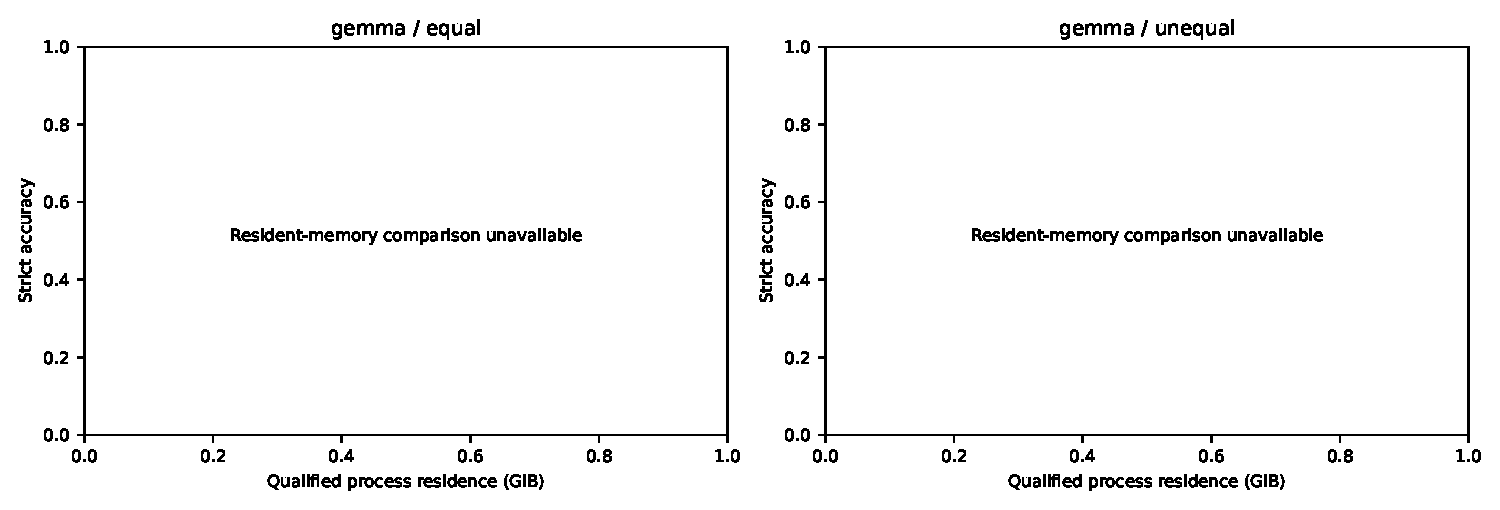
\includegraphics[width=\linewidth]{generated/research_campaign_v3/research-campaign-v3-20261012-r4/d2a1e138e22bcee13dbe650d6e2375b7d7300e7009a6cb4bc54c6b52f678c195/figures/gemma-memory.pdf}\caption{Accuracy versus measured resident memory; unavailable comparisons are explicit.}\end{figure}
\begin{figure}[htbp]\centering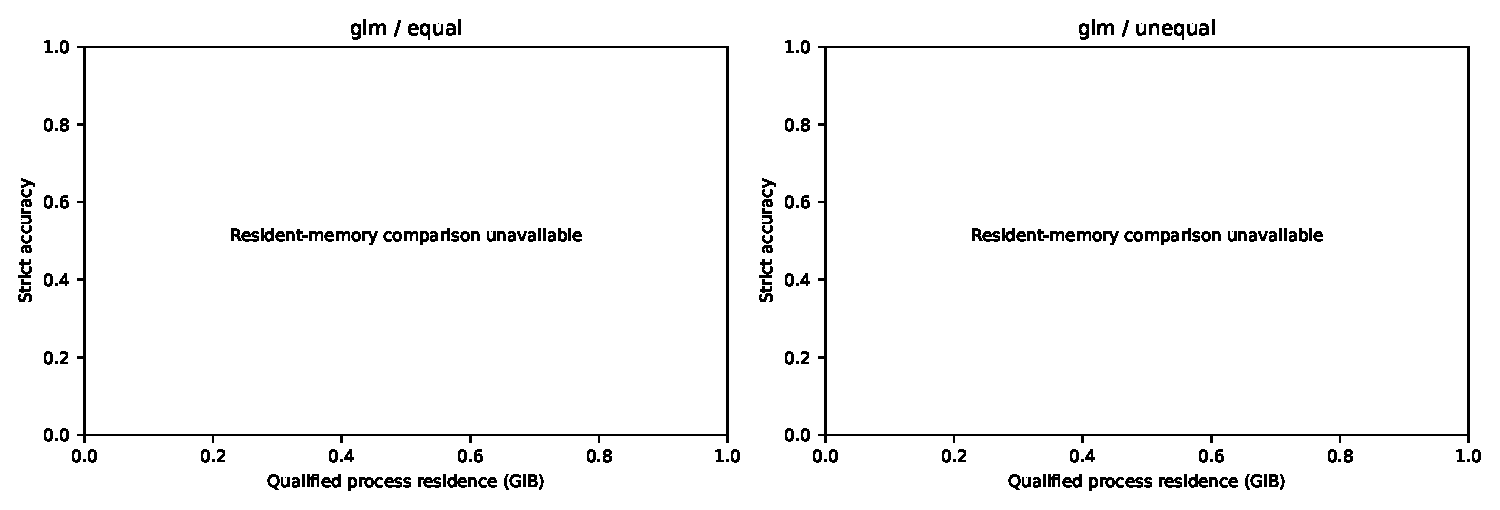
\includegraphics[width=\linewidth]{generated/research_campaign_v3/research-campaign-v3-20261012-r4/d2a1e138e22bcee13dbe650d6e2375b7d7300e7009a6cb4bc54c6b52f678c195/figures/glm-memory.pdf}\caption{Accuracy versus measured resident memory; unavailable comparisons are explicit.}\end{figure}
\begin{figure}[htbp]\centering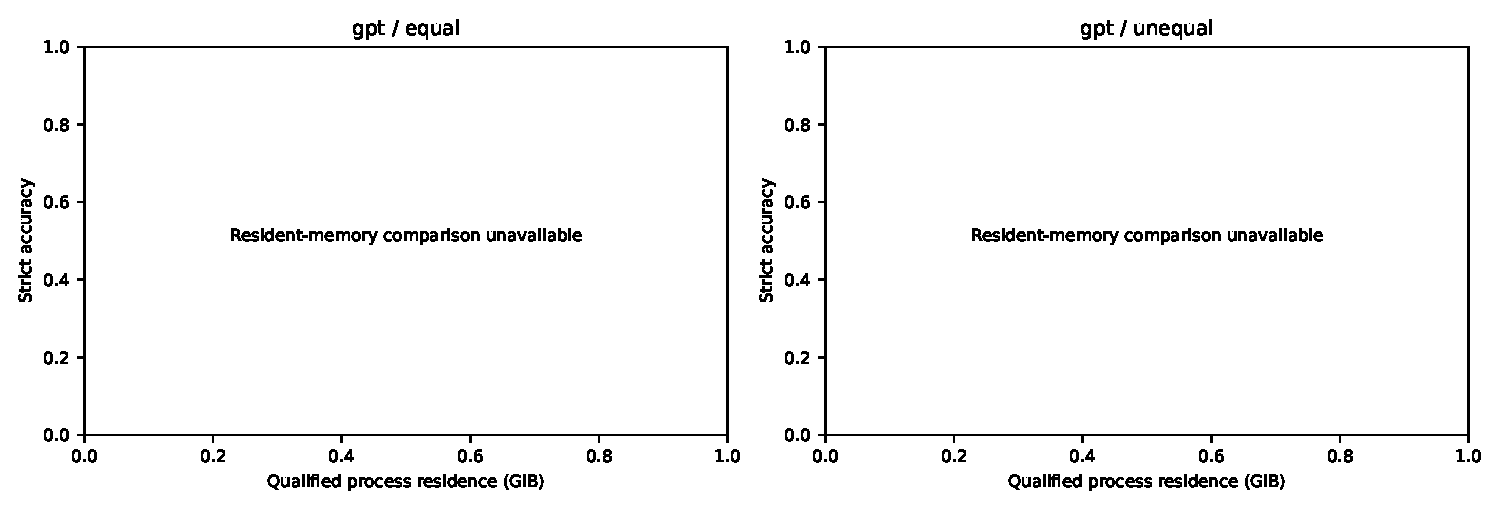
\includegraphics[width=\linewidth]{generated/research_campaign_v3/research-campaign-v3-20261012-r4/d2a1e138e22bcee13dbe650d6e2375b7d7300e7009a6cb4bc54c6b52f678c195/figures/gpt-memory.pdf}\caption{Accuracy versus measured resident memory; unavailable comparisons are explicit.}\end{figure}
\begin{figure}[htbp]\centering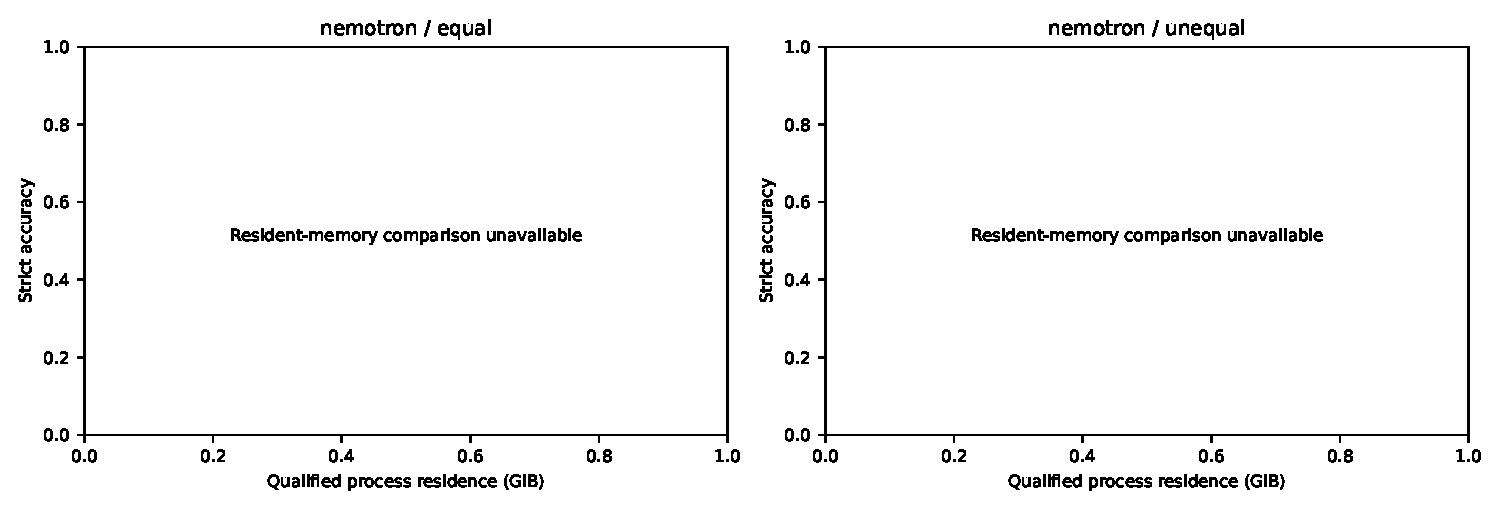
\includegraphics[width=\linewidth]{generated/research_campaign_v3/research-campaign-v3-20261012-r4/d2a1e138e22bcee13dbe650d6e2375b7d7300e7009a6cb4bc54c6b52f678c195/figures/nemotron-memory.pdf}\caption{Accuracy versus measured resident memory; unavailable comparisons are explicit.}\end{figure}
\begin{figure}[htbp]\centering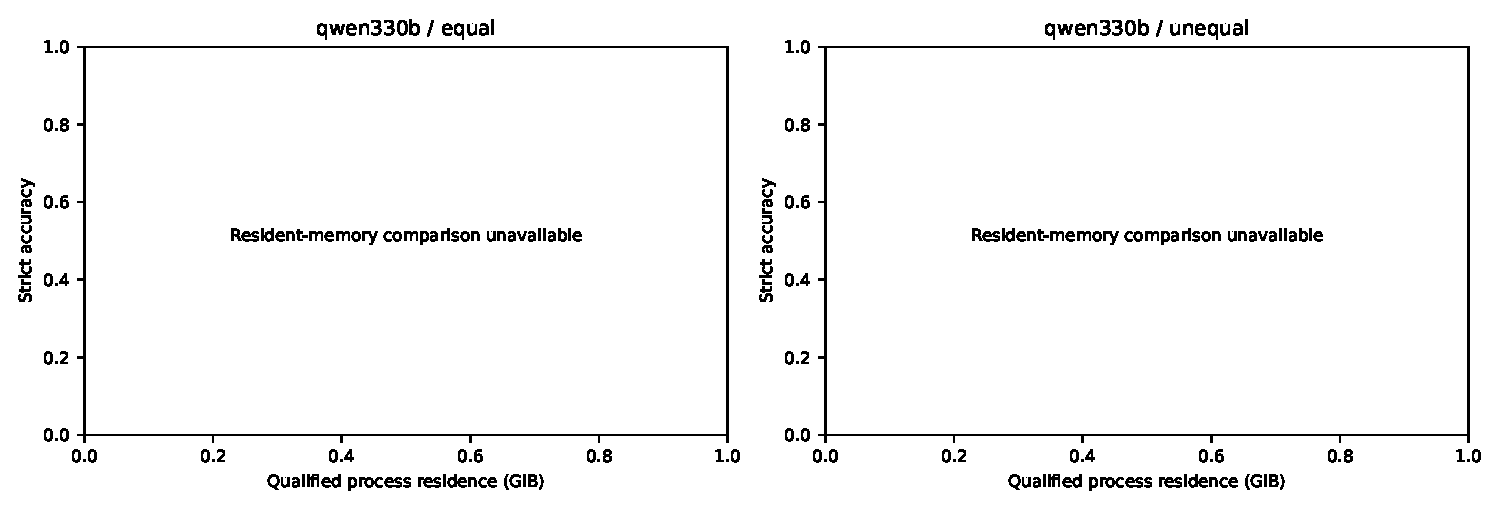
\includegraphics[width=\linewidth]{generated/research_campaign_v3/research-campaign-v3-20261012-r4/d2a1e138e22bcee13dbe650d6e2375b7d7300e7009a6cb4bc54c6b52f678c195/figures/qwen330b-memory.pdf}\caption{Accuracy versus measured resident memory; unavailable comparisons are explicit.}\end{figure}
\begin{figure}[htbp]\centering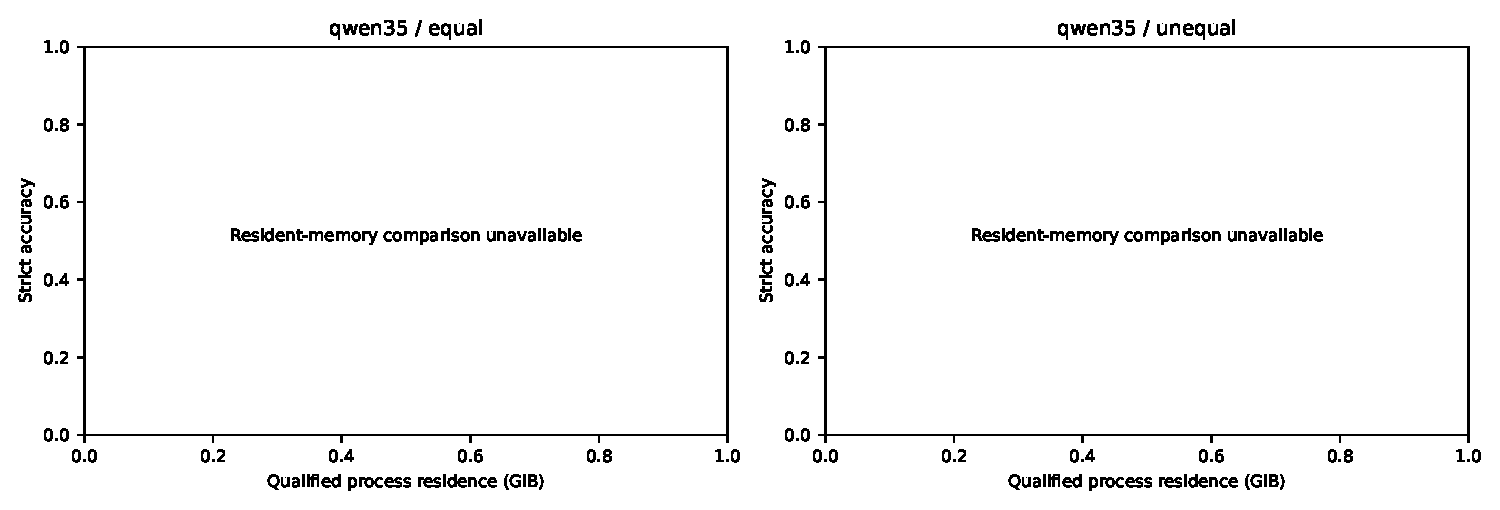
\includegraphics[width=\linewidth]{generated/research_campaign_v3/research-campaign-v3-20261012-r4/d2a1e138e22bcee13dbe650d6e2375b7d7300e7009a6cb4bc54c6b52f678c195/figures/qwen35-memory.pdf}\caption{Accuracy versus measured resident memory; unavailable comparisons are explicit.}\end{figure}
\begin{figure}[htbp]\centering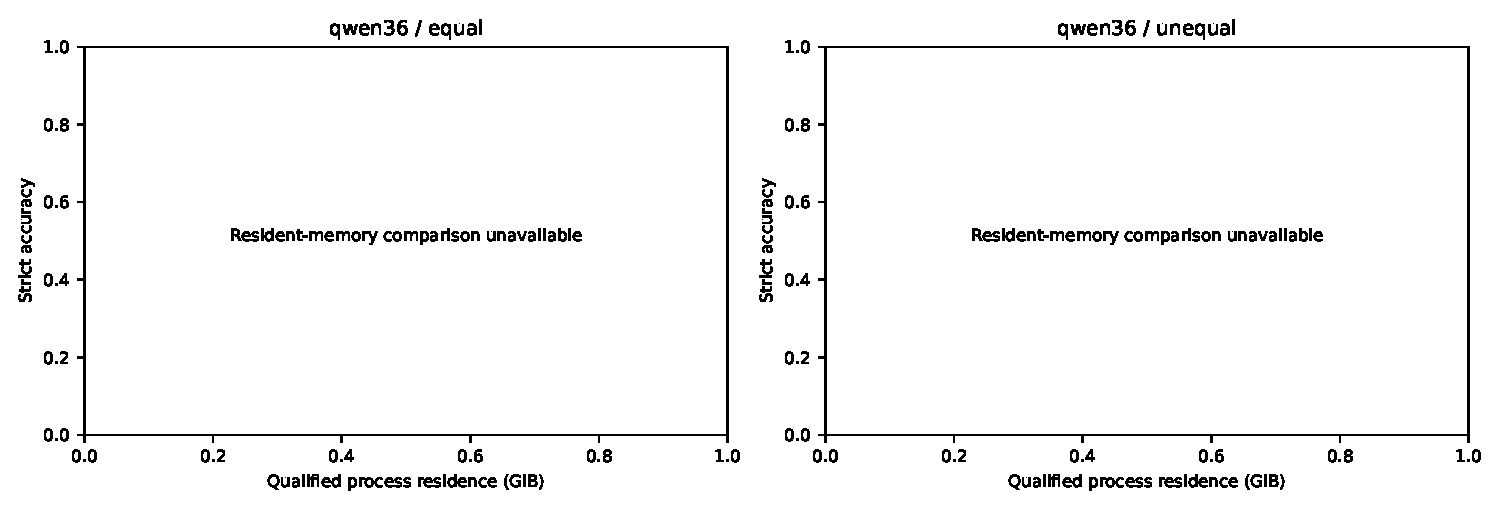
\includegraphics[width=\linewidth]{generated/research_campaign_v3/research-campaign-v3-20261012-r4/d2a1e138e22bcee13dbe650d6e2375b7d7300e7009a6cb4bc54c6b52f678c195/figures/qwen36-memory.pdf}\caption{Accuracy versus measured resident memory; unavailable comparisons are explicit.}\end{figure}
\subsection{Central steering}
The 129-family cohort retains all seven classes, three depths, both signs and native/random controls. First-complete-sentence response and post-pulse target occupancy share one simultaneous family over 1,176 contrasts and 2,352 bound components. Dwell, transitions, re-entry, recovery and target exits have separate supporting families; accuracy and tokens are reported jointly. Small or imprecise effects remain unresolved.\par
\begin{figure}[htbp]\centering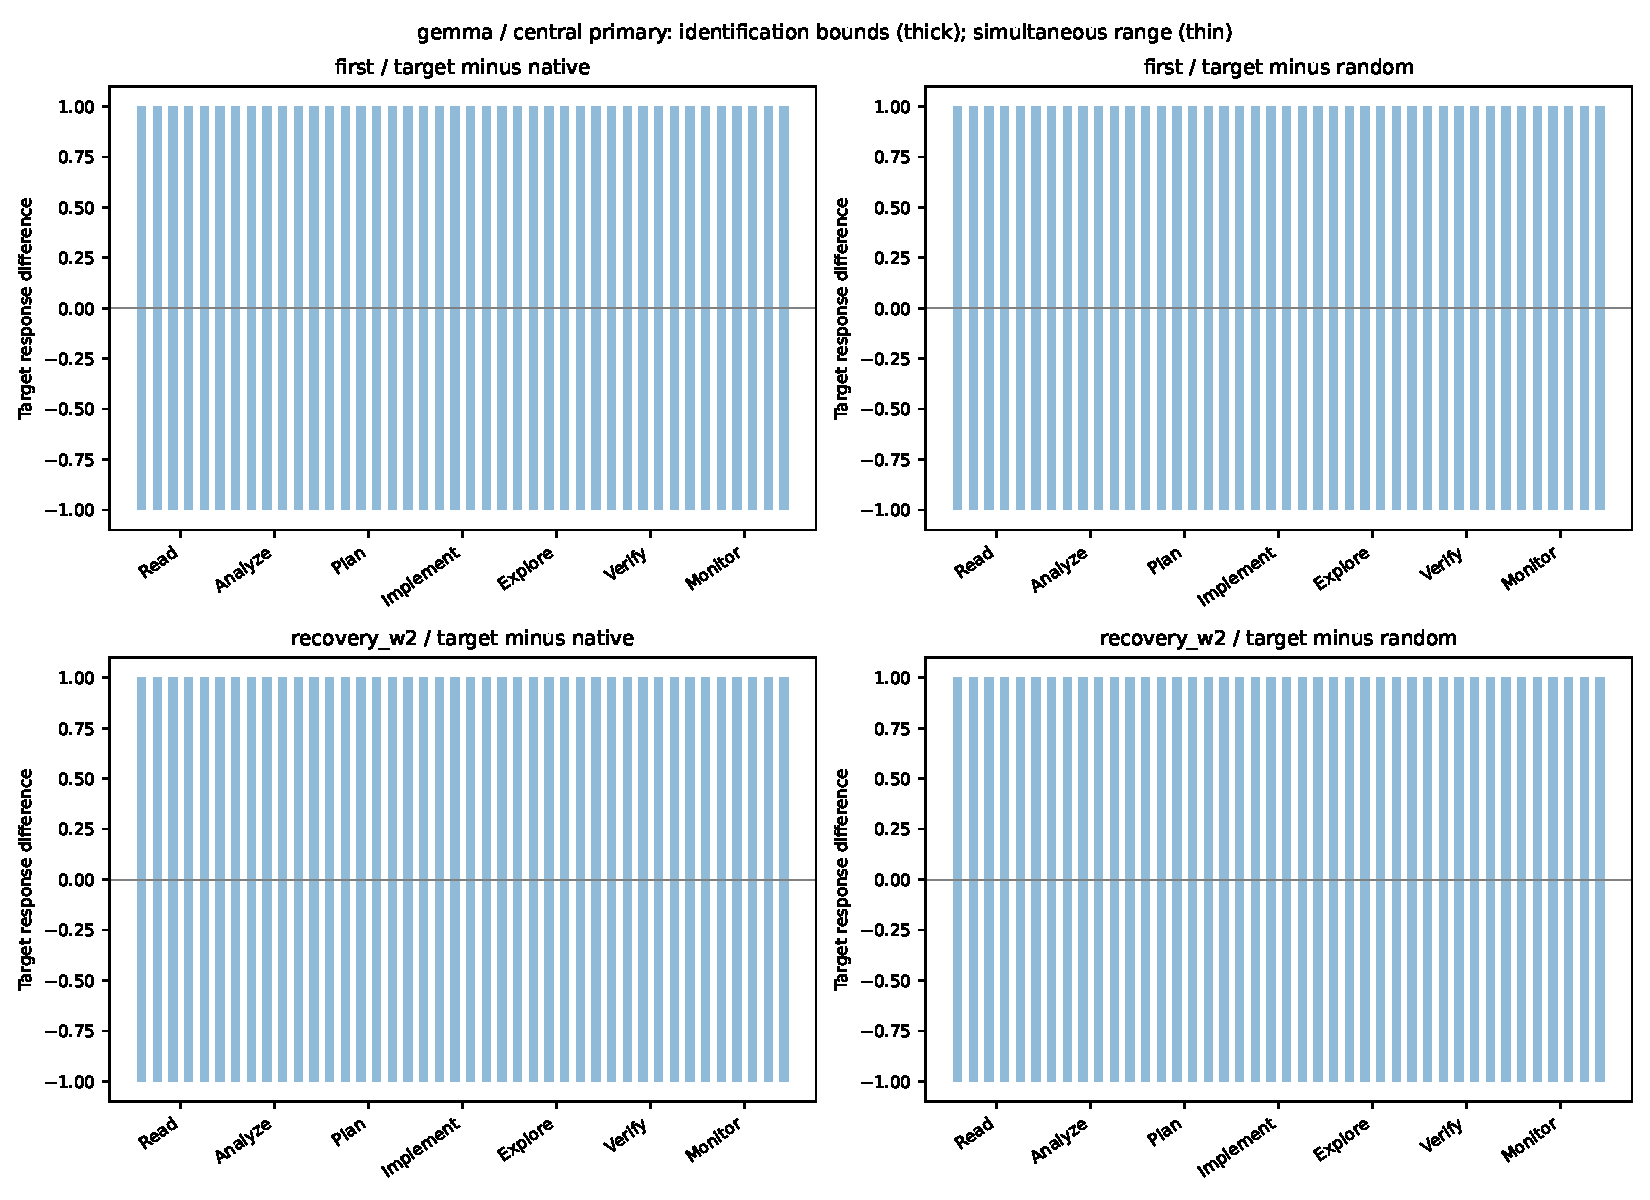
\includegraphics[width=\linewidth]{generated/research_campaign_v3/research-campaign-v3-20261012-r4/d2a1e138e22bcee13dbe650d6e2375b7d7300e7009a6cb4bc54c6b52f678c195/figures/gemma-central-primary.pdf}\caption{Central primary identification bounds and study-wide simultaneous uncertainty.}\end{figure}
\begin{figure}[htbp]\centering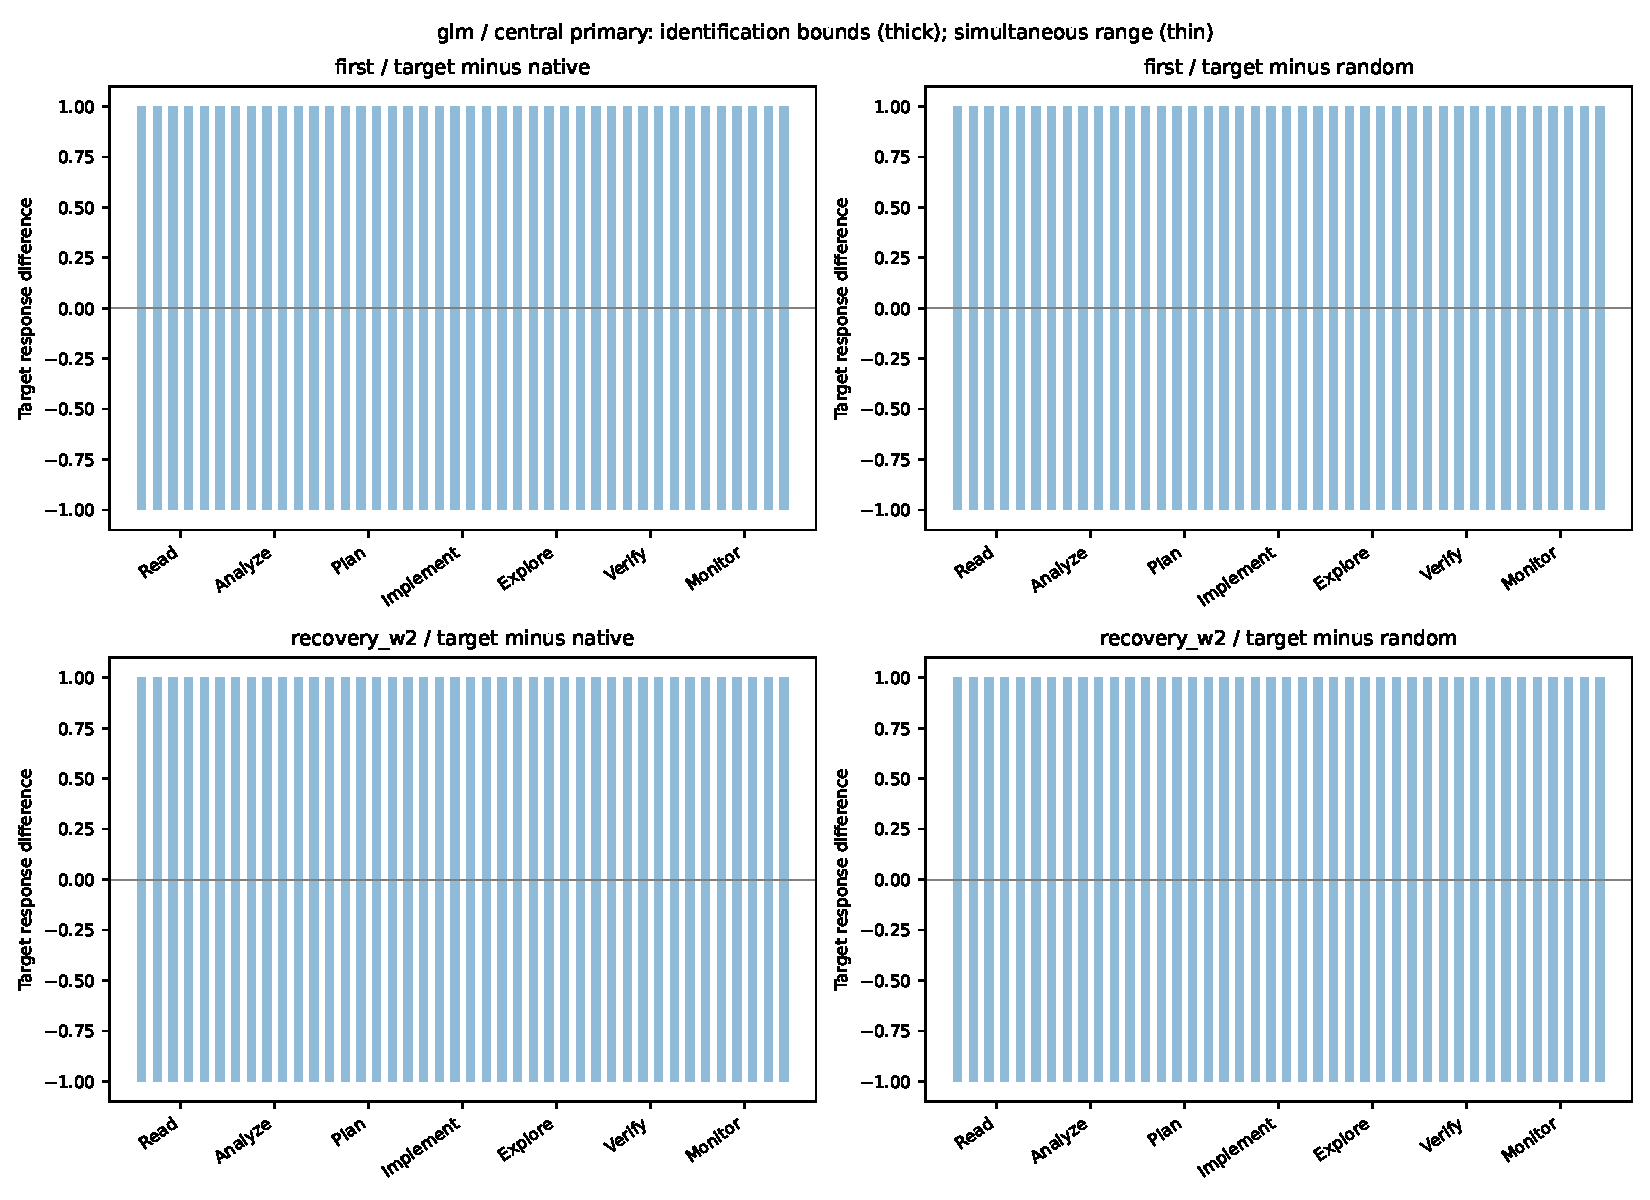
\includegraphics[width=\linewidth]{generated/research_campaign_v3/research-campaign-v3-20261012-r4/d2a1e138e22bcee13dbe650d6e2375b7d7300e7009a6cb4bc54c6b52f678c195/figures/glm-central-primary.pdf}\caption{Central primary identification bounds and study-wide simultaneous uncertainty.}\end{figure}
\begin{figure}[htbp]\centering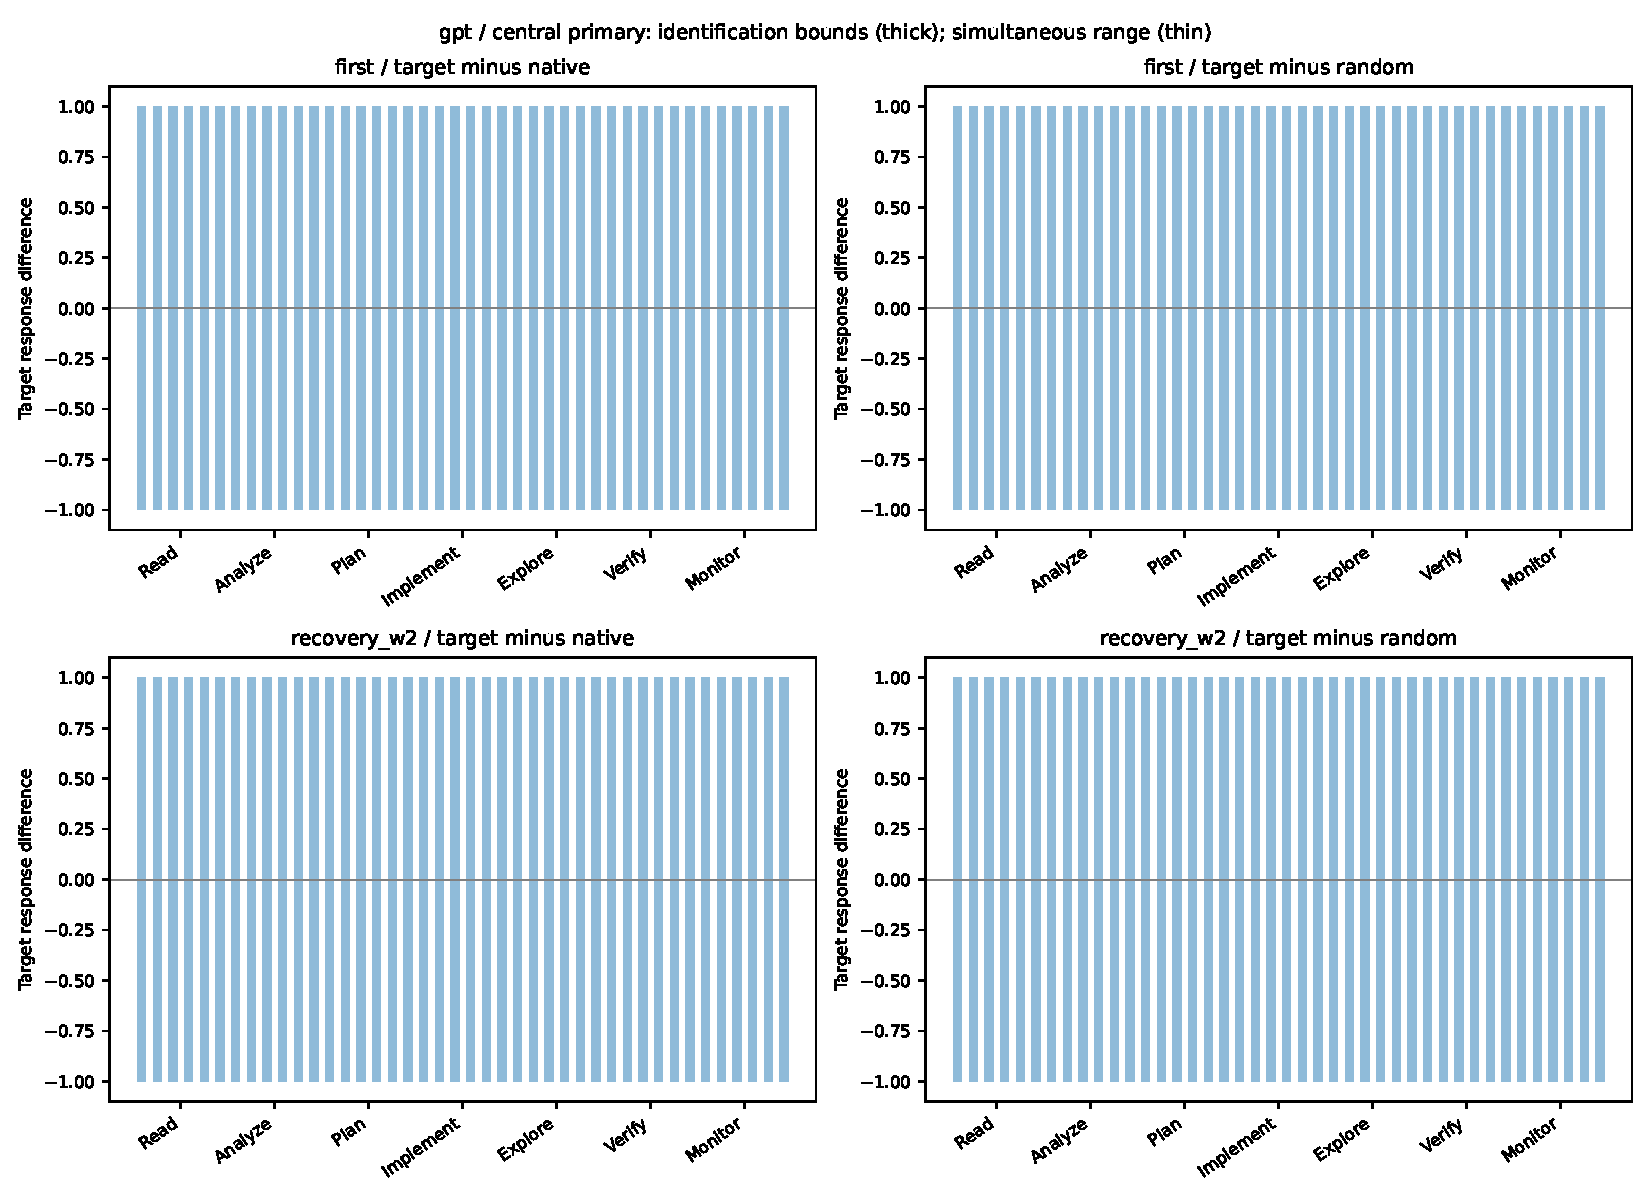
\includegraphics[width=\linewidth]{generated/research_campaign_v3/research-campaign-v3-20261012-r4/d2a1e138e22bcee13dbe650d6e2375b7d7300e7009a6cb4bc54c6b52f678c195/figures/gpt-central-primary.pdf}\caption{Central primary identification bounds and study-wide simultaneous uncertainty.}\end{figure}
\begin{figure}[htbp]\centering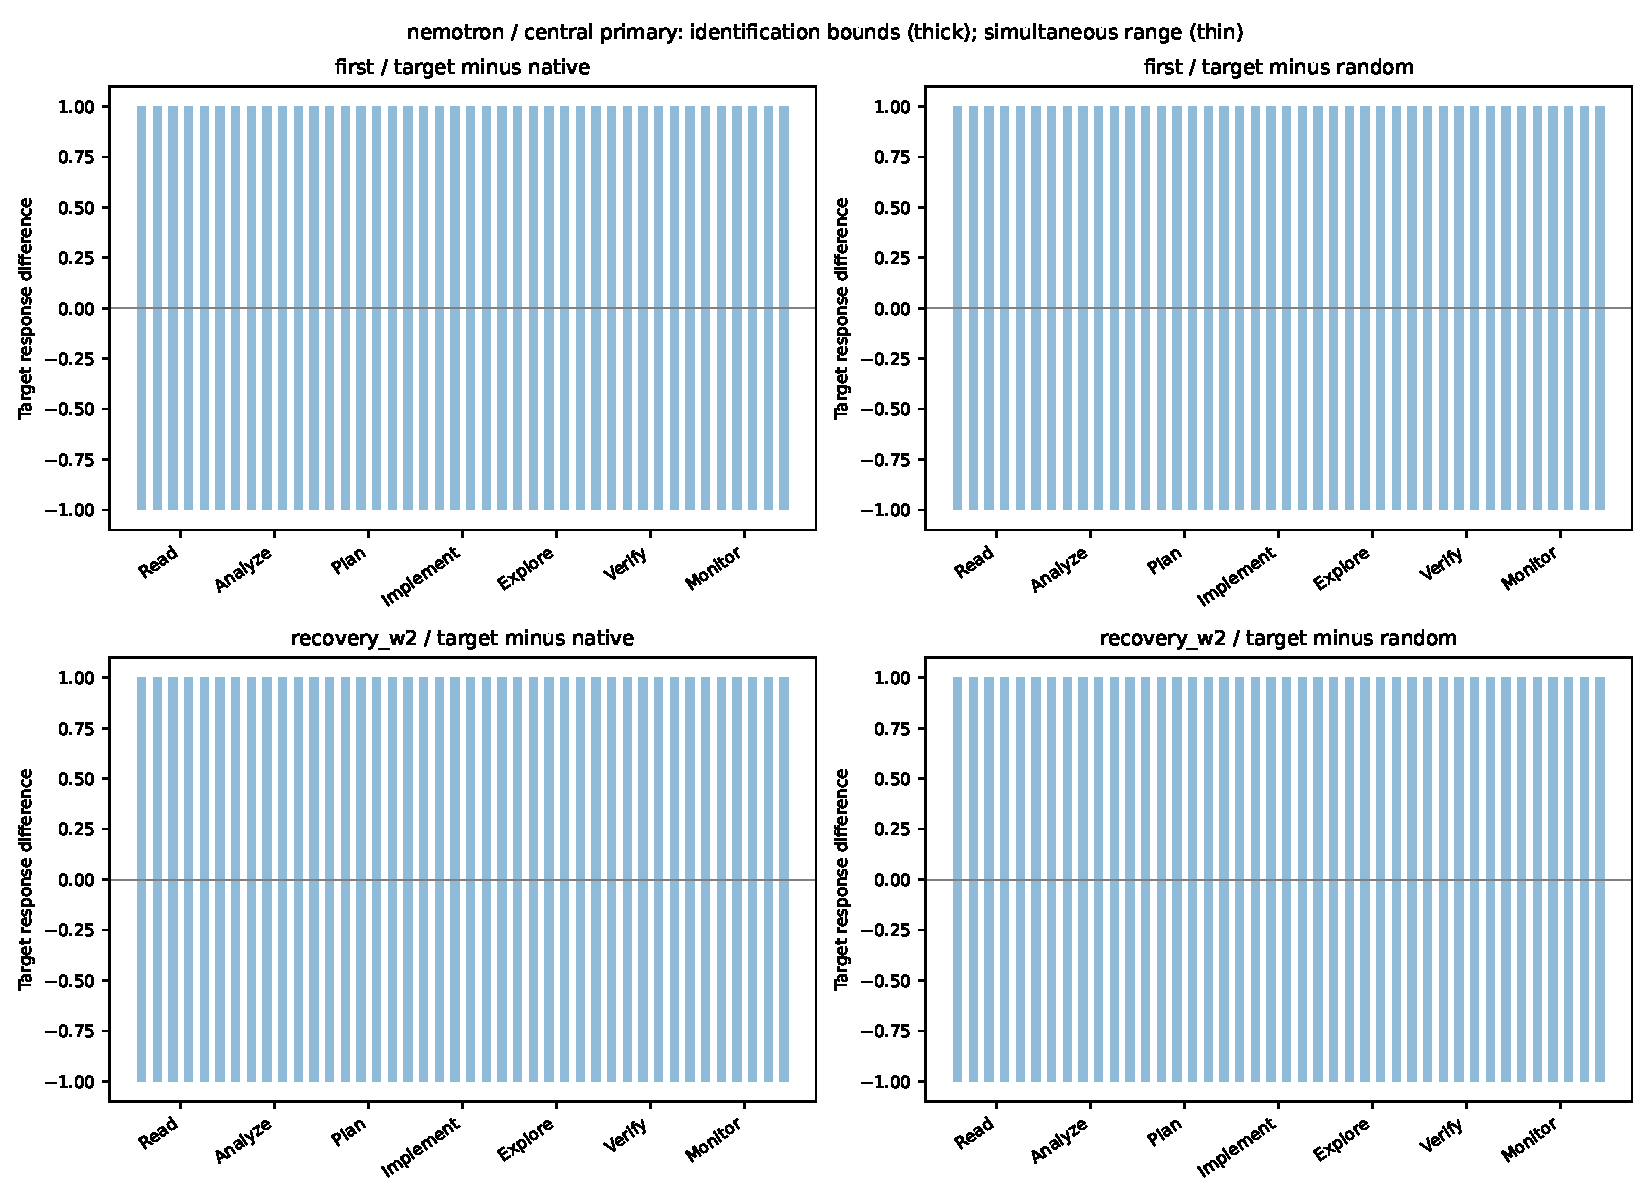
\includegraphics[width=\linewidth]{generated/research_campaign_v3/research-campaign-v3-20261012-r4/d2a1e138e22bcee13dbe650d6e2375b7d7300e7009a6cb4bc54c6b52f678c195/figures/nemotron-central-primary.pdf}\caption{Central primary identification bounds and study-wide simultaneous uncertainty.}\end{figure}
\begin{figure}[htbp]\centering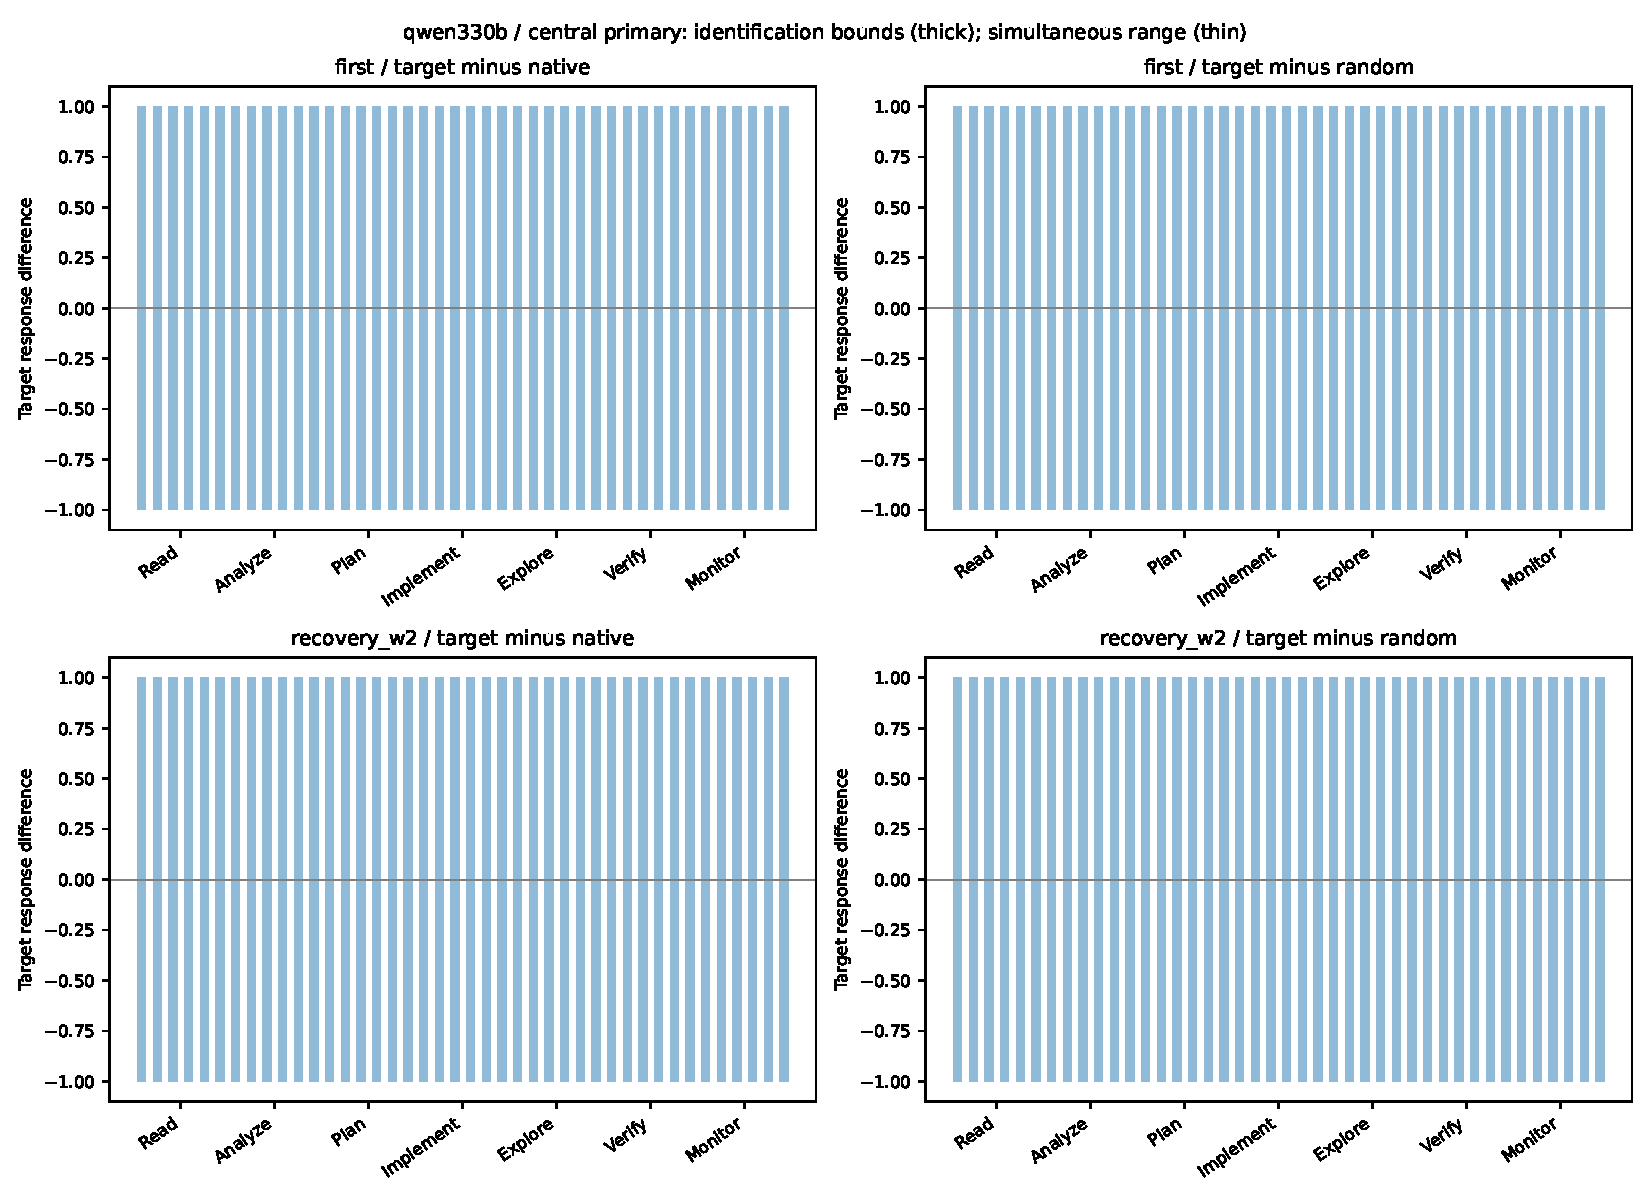
\includegraphics[width=\linewidth]{generated/research_campaign_v3/research-campaign-v3-20261012-r4/d2a1e138e22bcee13dbe650d6e2375b7d7300e7009a6cb4bc54c6b52f678c195/figures/qwen330b-central-primary.pdf}\caption{Central primary identification bounds and study-wide simultaneous uncertainty.}\end{figure}
\begin{figure}[htbp]\centering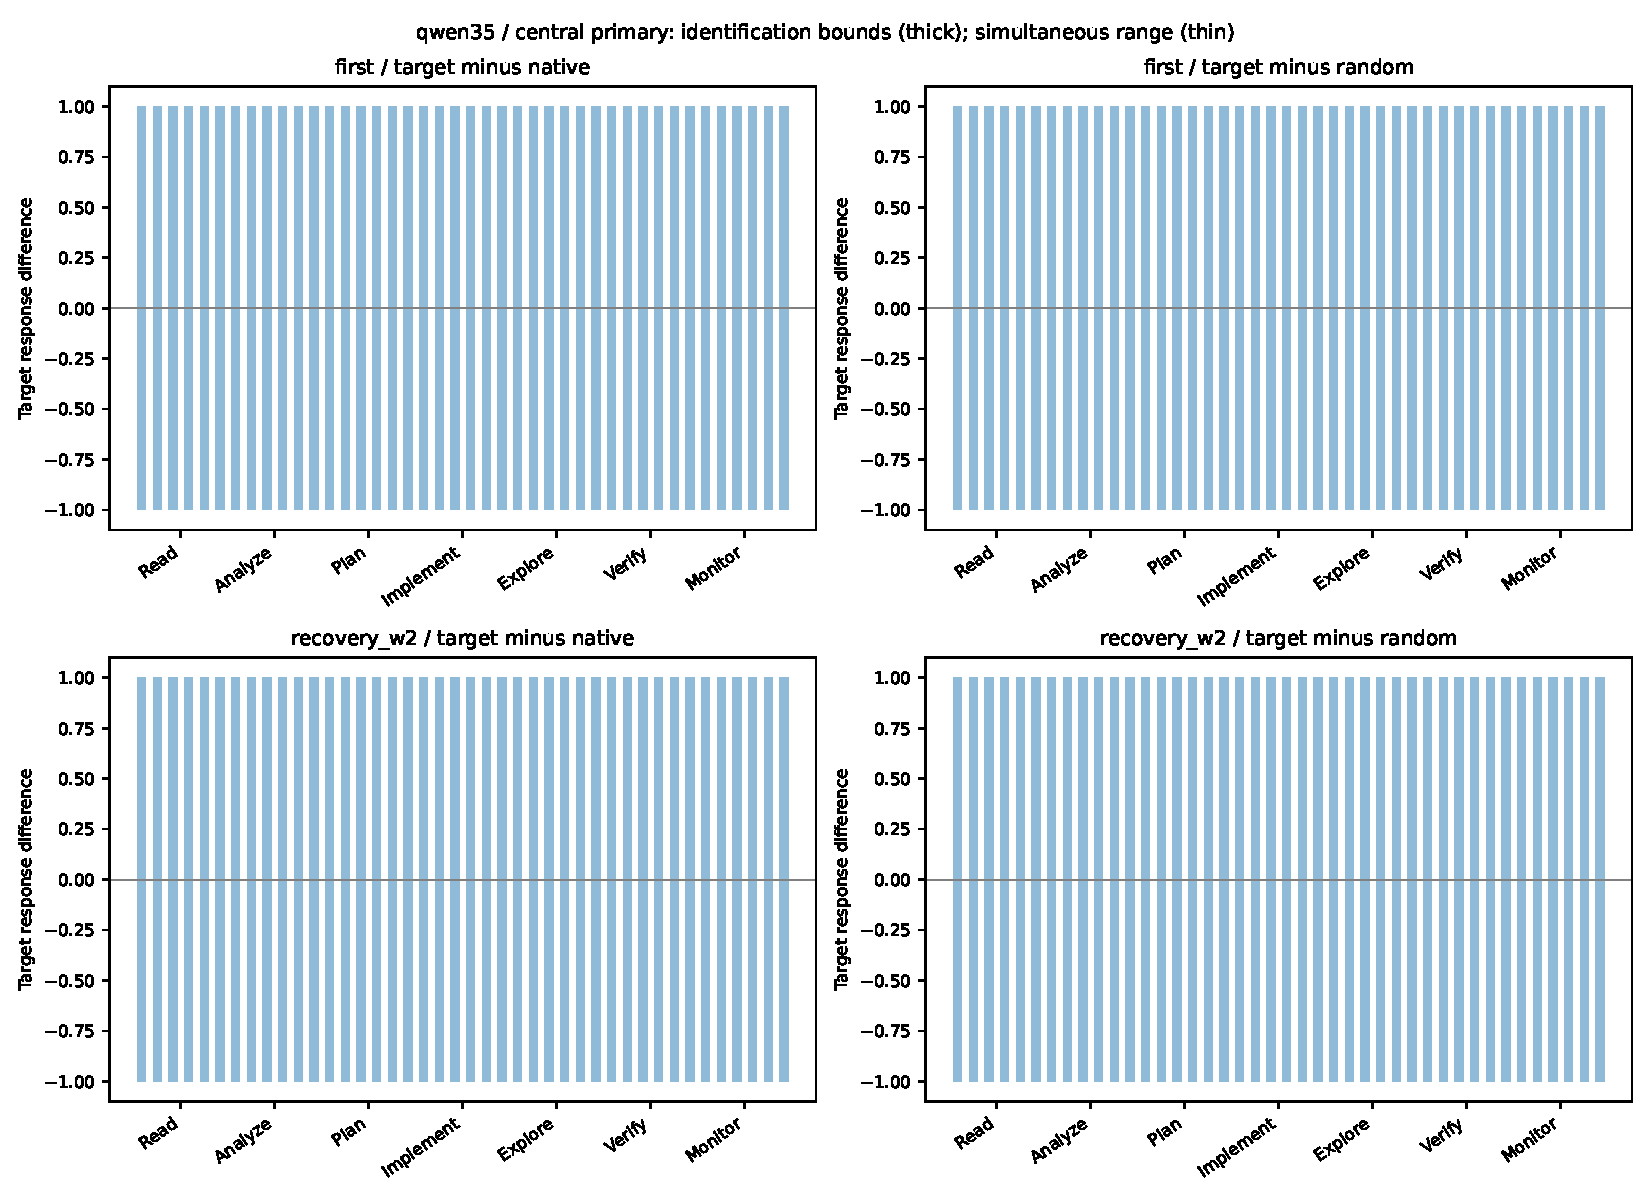
\includegraphics[width=\linewidth]{generated/research_campaign_v3/research-campaign-v3-20261012-r4/d2a1e138e22bcee13dbe650d6e2375b7d7300e7009a6cb4bc54c6b52f678c195/figures/qwen35-central-primary.pdf}\caption{Central primary identification bounds and study-wide simultaneous uncertainty.}\end{figure}
\begin{figure}[htbp]\centering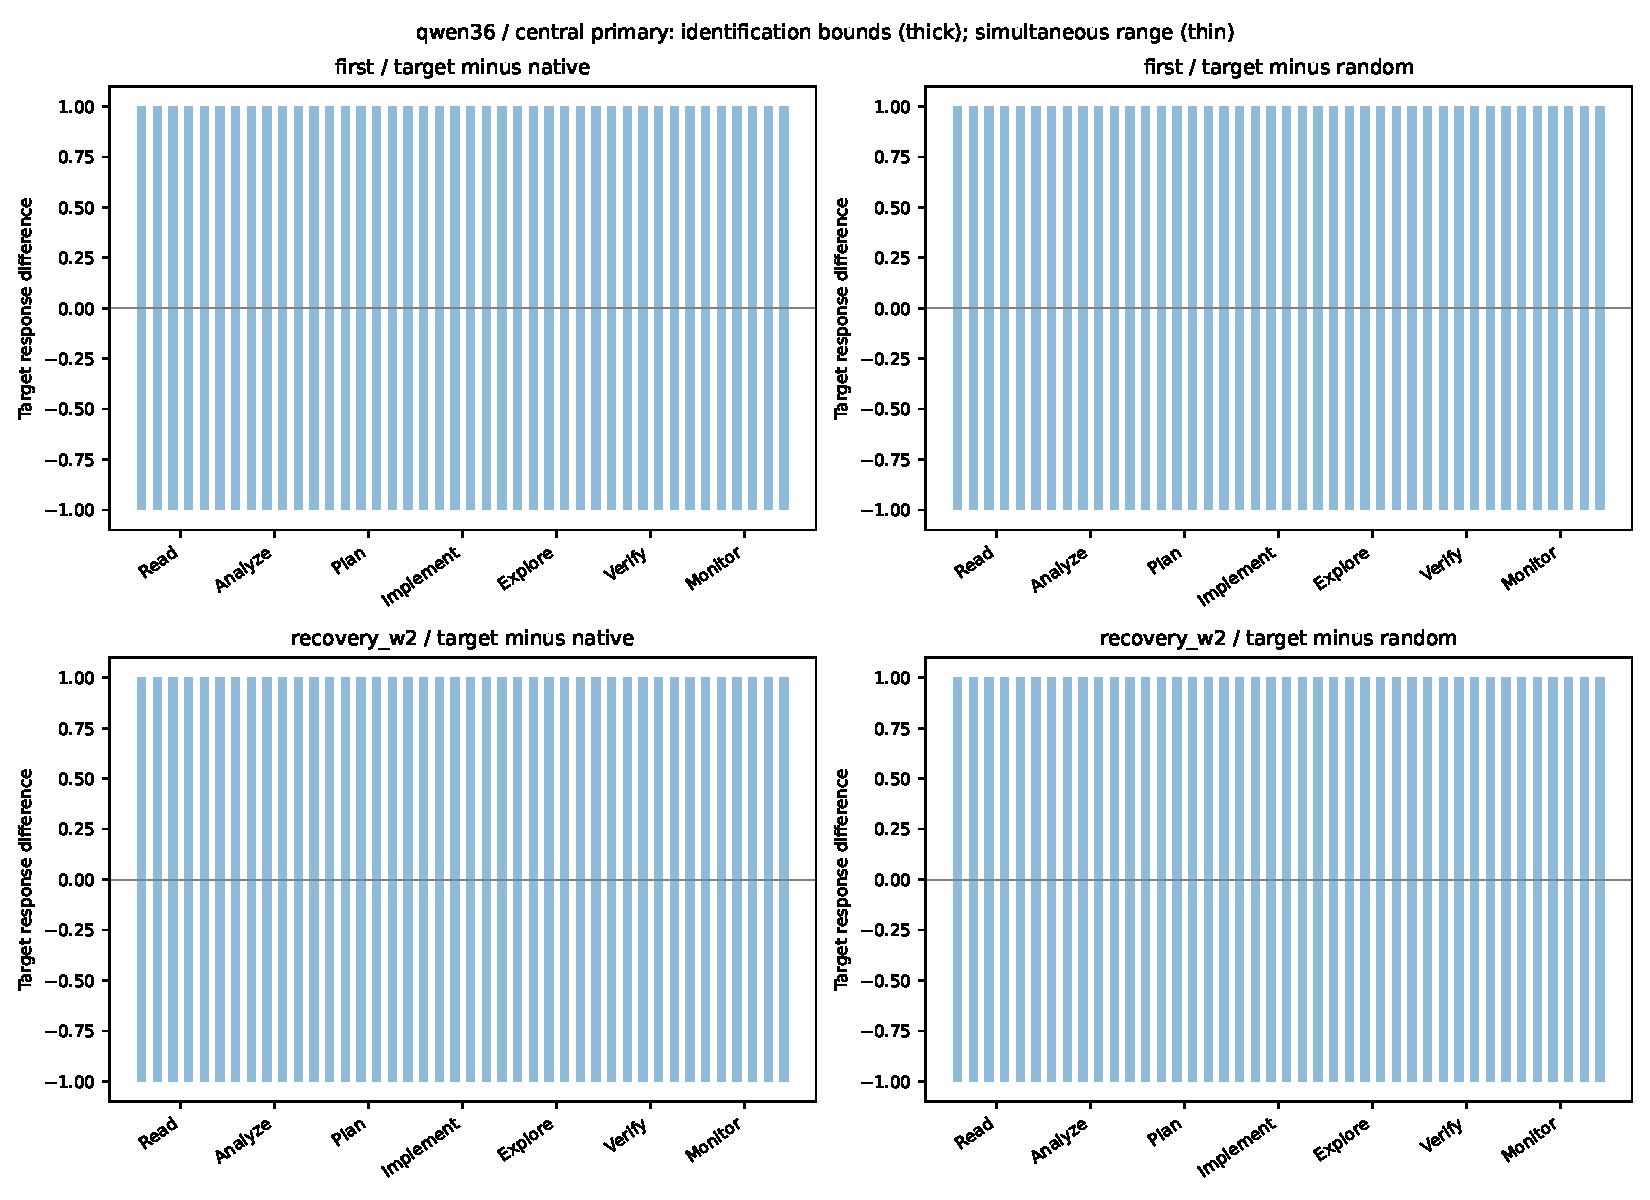
\includegraphics[width=\linewidth]{generated/research_campaign_v3/research-campaign-v3-20261012-r4/d2a1e138e22bcee13dbe650d6e2375b7d7300e7009a6cb4bc54c6b52f678c195/figures/qwen36-central-primary.pdf}\caption{Central primary identification bounds and study-wide simultaneous uncertainty.}\end{figure}
